\subsection{Comptonization of the CMB}

If we define the planck spectrum to be

\begin{equation}
I(x) = {{2(k_B T)^3}\over{(hc)^2}}{{x^3}\over{e^x - 1}} = i_0\,i(x), 
\end{equation}

then change in intensity due to inverse-Compton scattering of a
blackbody distribution of photons by an isotropic distribution of
electrons is given in the optically thin limit ($\tau \ll 1$) by:

\begin{equation}
\Delta i(x) \equiv {\Delta I(x)\over{i_0}} = \left\{j(x) - i(x)\right\}\tau
\label{eq:deltai}
\end{equation}

where

\begin{equation}
\tau = \sigma_T\integral{}{}{n_e}{\ell},
\end{equation}

is the optical depth, $i(x)\tau$ is the flux scattered to other frequencies and
$j(x)\tau$ is the flux scattered from other frequencies to $x =
h\nu/(kT)$. 

It is useful to rewrite Eq.~\ref{eq:deltai} as

\begin{equation}
\Delta i(x) = \tilde{g}(x)\,\tilde{y},
\end{equation}

where

\begin{eqnarray}\nonumber
\tilde{y} &=& {{\sigma_T}\over{m_e c^2}}\integral{}{}{n_e k_B \tilde{T}_e}{\ell}\\\nonumber
\end{eqnarray}

and $\tilde{T}_e$ is defined by 

\begin{equation}
k_B\tilde{T}_e = {{P_e}\over{n_e}}
\end{equation}

(in the case of a thermal distribution of electrons, $\tilde{T}_e \equiv T_e$).  Defining 

\begin{equation}
\left<k_B\tilde{T}_e\right> = {{\integral{}{}{n_ek_B\tilde{T}_e}{\ell}}\over{\integral{}{}{n_e}{\ell}}}
\end{equation}

we have

\begin{equation}
\tilde{g}(x) = \left\{j(x) - i(x)\right\}{{m_e c^2}\over{\left<k_B\tilde{T}_e\right>}}
\label{eq:ggen}
\end{equation}

For a thermal distribution of electrons, $\left<k_B\tilde{T}_e\right>
\equiv k_B T_e$, and in the non-relativistic regime, we have

\begin{equation}
\tilde{g}(x) = {{x^4e^x}\over{(e^x-1)^2}}\left(x{{e^x+1}\over{e^x-1}} - 4\right) {{m_e c^2}\over{k_B T_e}},
\label{eq:komp}
\end{equation}

i.e., the standard non-relativistic solution to the Kompaneets
equation.  To make contact with Eq.~\ref{eq:ynu}, we can identify the
frequency dependence of the SZ temperature decrement in the
non-relativistic case as the central term of Eq.~\ref{eq:komp}:

\begin{equation}
f(x) = x{{e^x+1}\over{e^x-1}} - 4.
\label{eq:fnu}
\end{equation}

In general, though, for an arbitrary electron momentum
distribution $f_e(p)$, we have:

\begin{equation}
\left<k_B\tilde{T}_e\right> = \integral{0}{\infty}{f_e(p) {1\over{3}}pv(p)m_e c}{p},
\end{equation}

where $p = \beta_e\gamma_e$ is the normalized electron momentum. The
scattered spectrum is now given by

\begin{equation}
j(x) = \integral{0}{\infty}{P(t)i(x/t)}{t},
\end{equation}

where $P(t)$ is the probability that a photon is scattered to a
frequency $t = \nu^\prime/\nu$ times its original frequency.  The
photon redistribution function can be written as

\begin{equation}
P(t) = \integral{0}{\infty}{f_e(p)P(t;p)}{p},
\end{equation}

where $P(t;p)$ is the redistribution function for a mono-energetic
electron distribution, which in the Thomson regime ($h\nu \ll \gamma_e
m_e c^2$) has an analytic solution

\begin{eqnarray}\nonumber
P(t;p) = &-& {{3|1-t|}\over{32p^6t}} [1 + (10 + 8p^2 + 4p^4)t + t^2]\\\nonumber
         &+& {{3(1+t)}\over{8p^5}}\left[{{3+3p^2 + p^4}\over{\sqrt{1+p^2}}} - {{3+2p^2}\over{2p}}(2{\rm\,arcsinh(p)} - \left|\ln{t}\right|)\right],
\end{eqnarray}

where $P(t;p) = 0$ for $|\ln{t}| > 2{\,\rm arcsinh(p)}$.

\begin{figure}[th]
\begin{center}
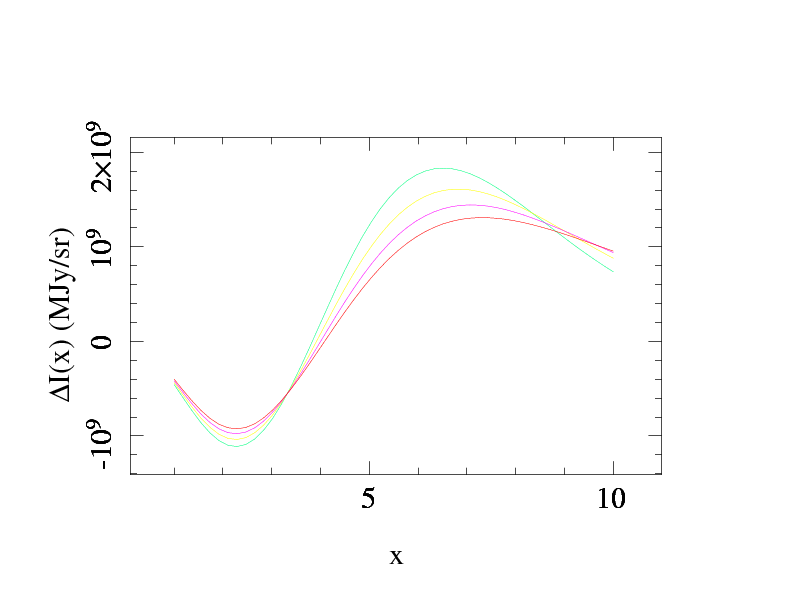
\includegraphics[scale=0.3]{figures/gx.png}\\
\end{center}
\caption{Comparison of the non-relativistic $\Delta I(x)$ computed with Eq.~\ref{eq:komp} (green) with the correct relativistic calculation using Eq.~\ref{eq:ggen}, for $T_e = 10, 20, 30~$keV.}
\label{fig:gx}
\end{figure}

